
%% bare_conf.tex
%% V1.4a
%% 2014/09/17
%% by Michael Shell
%% See:
%% http://www.michaelshell.org/
%% for current contact information.
%%
%% This is a skeleton file demonstrating the use of IEEEtran.cls
%% (requires IEEEtran.cls version 1.8a or later) with an IEEE
%% conference paper.
%%
%% Support sites:
%% http://www.michaelshell.org/tex/ieeetran/
%% http://www.ctan.org/tex-archive/macros/latex/contrib/IEEEtran/
%% and
%% http://www.ieee.org/

%%*************************************************************************
%% Legal Notice:
%% This code is offered as-is without any warranty either expressed or
%% implied; without even the implied warranty of MERCHANTABILITY or
%% FITNESS FOR A PARTICULAR PURPOSE! 
%% User assumes all risk.
%% In no event shall IEEE or any contributor to this code be liable for
%% any damages or losses, including, but not limited to, incidental,
%% consequential, or any other damages, resulting from the use or misuse
%% of any information contained here.
%%
%% All comments are the opinions of their respective authors and are not
%% necessarily endorsed by the IEEE.
%%
%% This work is distributed under the LaTeX Project Public License (LPPL)
%% ( http://www.latex-project.org/ ) version 1.3, and may be freely used,
%% distributed and modified. A copy of the LPPL, version 1.3, is included
%% in the base LaTeX documentation of all distributions of LaTeX released
%% 2003/12/01 or later.
%% Retain all contribution notices and credits.
%% ** Modified files should be clearly indicated as such, including  **
%% ** renaming them and changing author support contact information. **
%%
%% File list of work: IEEEtran.cls, IEEEtran_HOWTO.pdf, bare_adv.tex,
%%                    bare_conf.tex, bare_jrnl.tex, bare_conf_compsoc.tex,
%%                    bare_jrnl_compsoc.tex, bare_jrnl_transmag.tex
%%*************************************************************************


% *** Authors should verify (and, if needed, correct) their LaTeX system  ***
% *** with the testflow diagnostic prior to trusting their LaTeX platform ***
% *** with production work. IEEE's font choices and paper sizes can       ***
% *** trigger bugs that do not appear when using other class files.       ***                          ***
% The testflow support page is at:
% http://www.michaelshell.org/tex/testflow/



\documentclass[conference]{IEEEtran}
% Some Computer Society conferences also require the compsoc mode option,
% but others use the standard conference format.
%
% If IEEEtran.cls has not been installed into the LaTeX system files,
% manually specify the path to it like:
% \documentclass[conference]{../sty/IEEEtran}





% Some very useful LaTeX packages include:
% (uncomment the ones you want to load)


% *** MISC UTILITY PACKAGES ***
%
%\usepackage{ifpdf}
% Heiko Oberdiek's ifpdf.sty is very useful if you need conditional
% compilation based on whether the output is pdf or dvi.
% usage:
% \ifpdf
%   % pdf code
% \else
%   % dvi code
% \fi
% The latest version of ifpdf.sty can be obtained from:
% http://www.ctan.org/tex-archive/macros/latex/contrib/oberdiek/
% Also, note that IEEEtran.cls V1.7 and later provides a builtin
% \ifCLASSINFOpdf conditional that works the same way.
% When switching from latex to pdflatex and vice-versa, the compiler may
% have to be run twice to clear warning/error messages.






% *** CITATION PACKAGES ***
%
%\usepackage{cite}
% cite.sty was written by Donald Arseneau
% V1.6 and later of IEEEtran pre-defines the format of the cite.sty package
% \cite{} output to follow that of IEEE. Loading the cite package will
% result in citation numbers being automatically sorted and properly
% "compressed/ranged". e.g., [1], [9], [2], [7], [5], [6] without using
% cite.sty will become [1], [2], [5]--[7], [9] using cite.sty. cite.sty's
% \cite will automatically add leading space, if needed. Use cite.sty's
% noadjust option (cite.sty V3.8 and later) if you want to turn this off
% such as if a citation ever needs to be enclosed in parenthesis.
% cite.sty is already installed on most LaTeX systems. Be sure and use
% version 5.0 (2009-03-20) and later if using hyperref.sty.
% The latest version can be obtained at:
% http://www.ctan.org/tex-archive/macros/latex/contrib/cite/
% The documentation is contained in the cite.sty file itself.






% *** GRAPHICS RELATED PACKAGES ***
%
\ifCLASSINFOpdf
  % \usepackage[pdftex]{graphicx}
  % declare the path(s) where your graphic files are
  % \graphicspath{{../pdf/}{../jpeg/}}
  % and their extensions so you won't have to specify these with
  % every instance of \includegraphics
  % \DeclareGraphicsExtensions{.pdf,.jpeg,.png}
\else
  % or other class option (dvipsone, dvipdf, if not using dvips). graphicx
  % will default to the driver specified in the system graphics.cfg if no
  % driver is specified.
  % \usepackage[dvips]{graphicx}
  % declare the path(s) where your graphic files are
  % \graphicspath{{../eps/}}
  % and their extensions so you won't have to specify these with
  % every instance of \includegraphics
  % \DeclareGraphicsExtensions{.eps}
\fi
% graphicx was written by David Carlisle and Sebastian Rahtz. It is
% required if you want graphics, photos, etc. graphicx.sty is already
% installed on most LaTeX systems. The latest version and documentation
% can be obtained at: 
% http://www.ctan.org/tex-archive/macros/latex/required/graphics/
% Another good source of documentation is "Using Imported Graphics in
% LaTeX2e" by Keith Reckdahl which can be found at:
% http://www.ctan.org/tex-archive/info/epslatex/
%
% latex, and pdflatex in dvi mode, support graphics in encapsulated
% postscript (.eps) format. pdflatex in pdf mode supports graphics
% in .pdf, .jpeg, .png and .mps (metapost) formats. Users should ensure
% that all non-photo figures use a vector format (.eps, .pdf, .mps) and
% not a bitmapped formats (.jpeg, .png). IEEE frowns on bitmapped formats
% which can result in "jaggedy"/blurry rendering of lines and letters as
% well as large increases in file sizes.
%
% You can find documentation about the pdfTeX application at:
% http://www.tug.org/applications/pdftex





% *** MATH PACKAGES ***
%
\usepackage[cmex10]{amsmath}
\usepackage{amssymb}
\usepackage{mathtools}
% A popular package from the American Mathematical Society that provides
% many useful and powerful commands for dealing with mathematics. If using
% it, be sure to load this package with the cmex10 option to ensure that
% only type 1 fonts will utilized at all point sizes. Without this option,
% it is possible that some math symbols, particularly those within
% footnotes, will be rendered in bitmap form which will result in a
% document that can not be IEEE Xplore compliant!
%
% Also, note that the amsmath package sets \interdisplaylinepenalty to 10000
% thus preventing page breaks from occurring within multiline equations. Use:
%\interdisplaylinepenalty=2500
% after loading amsmath to restore such page breaks as IEEEtran.cls normally
% does. amsmath.sty is already installed on most LaTeX systems. The latest
% version and documentation can be obtained at:
% http://www.ctan.org/tex-archive/macros/latex/required/amslatex/math/





% *** SPECIALIZED LIST PACKAGES ***
%
%\usepackage{algorithmic}
% algorithmic.sty was written by Peter Williams and Rogerio Brito.
% This package provides an algorithmic environment fo describing algorithms.
% You can use the algorithmic environment in-text or within a figure
% environment to provide for a floating algorithm. Do NOT use the algorithm
% floating environment provided by algorithm.sty (by the same authors) or
% algorithm2e.sty (by Christophe Fiorio) as IEEE does not use dedicated
% algorithm float types and packages that provide these will not provide
% correct IEEE style captions. The latest version and documentation of
% algorithmic.sty can be obtained at:
% http://www.ctan.org/tex-archive/macros/latex/contrib/algorithms/
% There is also a support site at:
% http://algorithms.berlios.de/index.html
% Also of interest may be the (relatively newer and more customizable)
% algorithmicx.sty package by Szasz Janos:
% http://www.ctan.org/tex-archive/macros/latex/contrib/algorithmicx/




% *** ALIGNMENT PACKAGES ***
%
%\usepackage{array}
% Frank Mittelbach's and David Carlisle's array.sty patches and improves
% the standard LaTeX2e array and tabular environments to provide better
% appearance and additional user controls. As the default LaTeX2e table
% generation code is lacking to the point of almost being broken with
% respect to the quality of the end results, all users are strongly
% advised to use an enhanced (at the very least that provided by array.sty)
% set of table tools. array.sty is already installed on most systems. The
% latest version and documentation can be obtained at:
% http://www.ctan.org/tex-archive/macros/latex/required/tools/


% IEEEtran contains the IEEEeqnarray family of commands that can be used to
% generate multiline equations as well as matrices, tables, etc., of high
% quality.




% *** SUBFIGURE PACKAGES ***
%\ifCLASSOPTIONcompsoc
%  \usepackage[caption=false,font=normalsize,labelfont=sf,textfont=sf]{subfig}
%\else
%  \usepackage[caption=false,font=footnotesize]{subfig}
%\fi
% subfig.sty, written by Steven Douglas Cochran, is the modern replacement
% for subfigure.sty, the latter of which is no longer maintained and is
% incompatible with some LaTeX packages including fixltx2e. However,
% subfig.sty requires and automatically loads Axel Sommerfeldt's caption.sty
% which will override IEEEtran.cls' handling of captions and this will result
% in non-IEEE style figure/table captions. To prevent this problem, be sure
% and invoke subfig.sty's "caption=false" package option (available since
% subfig.sty version 1.3, 2005/06/28) as this is will preserve IEEEtran.cls
% handling of captions.
% Note that the Computer Society format requires a larger sans serif font
% than the serif footnote size font used in traditional IEEE formatting
% and thus the need to invoke different subfig.sty package options depending
% on whether compsoc mode has been enabled.
%
% The latest version and documentation of subfig.sty can be obtained at:
% http://www.ctan.org/tex-archive/macros/latex/contrib/subfig/




% *** FLOAT PACKAGES ***
%
%\usepackage{fixltx2e}
% fixltx2e, the successor to the earlier fix2col.sty, was written by
% Frank Mittelbach and David Carlisle. This package corrects a few problems
% in the LaTeX2e kernel, the most notable of which is that in current
% LaTeX2e releases, the ordering of single and double column floats is not
% guaranteed to be preserved. Thus, an unpatched LaTeX2e can allow a
% single column figure to be placed prior to an earlier double column
% figure. The latest version and documentation can be found at:
% http://www.ctan.org/tex-archive/macros/latex/base/


%\usepackage{stfloats}
% stfloats.sty was written by Sigitas Tolusis. This package gives LaTeX2e
% the ability to do double column floats at the bottom of the page as well
% as the top. (e.g., "\begin{figure*}[!b]" is not normally possible in
% LaTeX2e). It also provides a command:
%\fnbelowfloat
% to enable the placement of footnotes below bottom floats (the standard
% LaTeX2e kernel puts them above bottom floats). This is an invasive package
% which rewrites many portions of the LaTeX2e float routines. It may not work
% with other packages that modify the LaTeX2e float routines. The latest
% version and documentation can be obtained at:
% http://www.ctan.org/tex-archive/macros/latex/contrib/sttools/
% Do not use the stfloats baselinefloat ability as IEEE does not allow
% \baselineskip to stretch. Authors submitting work to the IEEE should note
% that IEEE rarely uses double column equations and that authors should try
% to avoid such use. Do not be tempted to use the cuted.sty or midfloat.sty
% packages (also by Sigitas Tolusis) as IEEE does not format its papers in
% such ways.
% Do not attempt to use stfloats with fixltx2e as they are incompatible.
% Instead, use Morten Hogholm'a dblfloatfix which combines the features
% of both fixltx2e and stfloats:
%
% \usepackage{dblfloatfix}
% The latest version can be found at:
% http://www.ctan.org/tex-archive/macros/latex/contrib/dblfloatfix/




% *** PDF, URL AND HYPERLINK PACKAGES ***
%
%\usepackage{url}
% url.sty was written by Donald Arseneau. It provides better support for
% handling and breaking URLs. url.sty is already installed on most LaTeX
% systems. The latest version and documentation can be obtained at:
% http://www.ctan.org/tex-archive/macros/latex/contrib/url/
% Basically, \url{my_url_here}.




% *** Do not adjust lengths that control margins, column widths, etc. ***
% *** Do not use packages that alter fonts (such as pslatex).         ***
% There should be no need to do such things with IEEEtran.cls V1.6 and later.
% (Unless specifically asked to do so by the journal or conference you plan
% to submit to, of course. )


% correct bad hyphenation here
\hyphenation{op-tical net-works semi-conduc-tor}

\usepackage{hyperref}

\usepackage[utf8]{inputenc}

% Font and Fontencoding Magic
% FAQ: 
% http://tex.stackexchange.com/questions/664/why-should-i-use-usepackaget1fontenc
% http://en.wikipedia.org/wiki/Computer_Modern
% http://tex.stackexchange.com/questions/1390/latin-modern-vs-cm-super
\usepackage[T1]{fontenc}
\usepackage{lmodern}

\usepackage[protrusion=true,expansion=true,auto=true,tracking=true]{microtype}

\usepackage{cleveref}

% For graphics
\usepackage{graphicx}
\graphicspath{{../figures/}}

% to use Tikz for figures
\usepackage{tikz}
\usepackage{pgfplots}
\usetikzlibrary{shapes,arrows,3d,calc,fit,shadows,decorations,automata,backgrounds,petri,positioning}
\usepackage{xargs}
\newcommandx*{\includetikz}[3][1=\linewidth,2=0.3\linewidth]{
 \newlength{\fwidth}
 \setlength{\fwidth}{#1}
 \newlength{\fheight}
 \setlength{\fheight}{#2}
 \input{#3}
 \global\let\fwidth\undefined
 \global\let\fheight\undefined
}

\begin{document}
%
% paper title
% Titles are generally capitalized except for words such as a, an, and, as,
% at, but, by, for, in, nor, of, on, or, the, to and up, which are usually
% not capitalized unless they are the first or last word of the title.
% Linebreaks \\ can be used within to get better formatting as desired.
% Do not put math or special symbols in the title.
\title{Group Project: Image Guided \\Robotic Transcranial Magnetic Stimulation}


% author names and affiliations
% use a multiple column layout for up to three different
% affiliations
\author{\IEEEauthorblockN{Christopher Göthel, Gunnar Maerker, Fabian Sabljak, \\Jan-Philipp Scheel, Aashik Udupi}
\IEEEauthorblockA{Institute of Medical Technology at Hamburg University of Technology,\\ Am Schwarzenberg-Campus 3, 21073 Hamburg, Germany}
}

% conference papers do not typically use \thanks and this command
% is locked out in conference mode. If really needed, such as for
% the acknowledgment of grants, issue a \IEEEoverridecommandlockouts
% after \documentclass

% for over three affiliations, or if they all won't fit within the width
% of the page, use this alternative format:
% 
%\author{\IEEEauthorblockN{Michael Shell\IEEEauthorrefmark{1},
%Homer Simpson\IEEEauthorrefmark{2},
%James Kirk\IEEEauthorrefmark{3}, 
%Montgomery Scott\IEEEauthorrefmark{3} and
%Eldon Tyrell\IEEEauthorrefmark{4}}
%\IEEEauthorblockA{\IEEEauthorrefmark{1}School of Electrical and Computer Engineering\\
%Georgia Institute of Technology,
%Atlanta, Georgia 30332--0250\\ Email: see http://www.michaelshell.org/contact.html}
%\IEEEauthorblockA{\IEEEauthorrefmark{2}Twentieth Century Fox, Springfield, USA\\
%Email: homer@thesimpsons.com}
%\IEEEauthorblockA{\IEEEauthorrefmark{3}Starfleet Academy, San Francisco, California 96678-2391\\
%Telephone: (800) 555--1212, Fax: (888) 555--1212}
%\IEEEauthorblockA{\IEEEauthorrefmark{4}Tyrell Inc., 123 Replicant Street, Los Angeles, California 90210--4321}}




% use for special paper notices
%\IEEEspecialpapernotice{(Invited Paper)}




% make the title area
\maketitle

% As a general rule, do not put math, special symbols or citations
% in the abstract
\begin{abstract}
This report contains the results and approaches of the group work on the project of "Robotics and Navigation in Medicine". The task was to support transcranial magnetic stimulation (TMS) by a vision-guided robot which should compensate head movement. 
\end{abstract}

% no keywords




% For peer review papers, you can put extra information on the cover
% page as needed:
% \ifCLASSOPTIONpeerreview
% \begin{center} \bfseries EDICS Category: 3-BBND \end{center}
% \fi
%
% For peerreview papers, this IEEEtran command inserts a page break and
% creates the second title. It will be ignored for other modes.
\IEEEpeerreviewmaketitle



\section{Introduction}
% no \IEEEPARstart
Transcranial magnetic stimulation is used as a therapeutic and diagnostic technique. A magnetic coil needs to be placed for stimulation of a specific cortex. Therefore, compensation of patient movement is needed. During the group project, we developed a motion compensation system which is based on ROS and used both C++ and Python.



% An example of a floating figure using the graphicx package.
% Note that \label must occur AFTER (or within) \caption.
% For figures, \caption should occur after the \includegraphics.
% Note that IEEEtran v1.7 and later has special internal code that
% is designed to preserve the operation of \label within \caption
% even when the captionsoff option is in effect. However, because
% of issues like this, it may be the safest practice to put all your
% \label just after \caption rather than within \caption{}.
%
% Reminder: the "draftcls" or "draftclsnofoot", not "draft", class
% option should be used if it is desired that the figures are to be
% displayed while in draft mode.
%
%\begin{figure}[!t]
%\centering
%\includegraphics[width=2.5in]{myfigure}
% where an .eps filename suffix will be assumed under latex, 
% and a .pdf suffix will be assumed for pdflatex; or what has been declared
% via \DeclareGraphicsExtensions.
%\caption{Simulation results for the network.}
%\label{fig_sim}
%\end{figure}

% Note that IEEE typically puts floats only at the top, even when this
% results in a large percentage of a column being occupied by floats.


% An example of a double column floating figure using two subfigures.
% (The subfig.sty package must be loaded for this to work.)
% The subfigure \label commands are set within each subfloat command,
% and the \label for the overall figure must come after \caption.
% \hfil is used as a separator to get equal spacing.
% Watch out that the combined width of all the subfigures on a 
% line do not exceed the text width or a line break will occur.
%
%\begin{figure*}[!t]
%\centering
%\subfloat[Case I]{\includegraphics[width=2.5in]{box}%
%\label{fig_first_case}}
%\hfil
%\subfloat[Case II]{\includegraphics[width=2.5in]{box}%
%\label{fig_second_case}}
%\caption{Simulation results for the network.}
%\label{fig_sim}
%\end{figure*}
%
% Note that often IEEE papers with subfigures do not employ subfigure
% captions (using the optional argument to \subfloat[]), but instead will
% reference/describe all of them (a), (b), etc., within the main caption.
% Be aware that for subfig.sty to generate the (a), (b), etc., subfigure
% labels, the optional argument to \subfloat must be present. If a
% subcaption is not desired, just leave its contents blank,
% e.g., \subfloat[].


% An example of a floating table. Note that, for IEEE style tables, the
% \caption command should come BEFORE the table and, given that table
% captions serve much like titles, are usually capitalized except for words
% such as a, an, and, as, at, but, by, for, in, nor, of, on, or, the, to
% and up, which are usually not capitalized unless they are the first or
% last word of the caption. Table text will default to \footnotesize as
% IEEE normally uses this smaller font for tables.
% The \label must come after \caption as always.
%
%\begin{table}[!t]
%% increase table row spacing, adjust to taste
%\renewcommand{\arraystretch}{1.3}
% if using array.sty, it might be a good idea to tweak the value of
% \extrarowheight as needed to properly center the text within the cells
%\caption{An Example of a Table}
%\label{table_example}
%\centering
%% Some packages, such as MDW tools, offer better commands for making tables
%% than the plain LaTeX2e tabular which is used here.
%\begin{tabular}{|c||c|}
%\hline
%One & Two\\
%\hline
%Three & Four\\
%\hline
%\end{tabular}
%\end{table}


% Note that the IEEE does not put floats in the very first column
% - or typically anywhere on the first page for that matter. Also,
% in-text middle ("here") positioning is typically not used, but it
% is allowed and encouraged for Computer Society conferences (but
% not Computer Society journals). Most IEEE journals/conferences use
% top floats exclusively. 
% Note that, LaTeX2e, unlike IEEE journals/conferences, places
% footnotes above bottom floats. This can be corrected via the
% \fnbelowfloat command of the stfloats package.


\section{Tasks}
In this report, we will follow the structure of the project. It was sectioned into four parts: The kinematics of the robot, the calibration of the camera, the head pose estimation and the head movement compensation.
\subsection{Robot Kinematics - AU, GM}
In transcranial magnetic simulation procedure, for effective therapy, the motion of the head must be compensated by moving the magnetic coil held by the robot end-effector. Thus, understanding the robot motion is crucial in solving such a task. This is possible by solving the direct kinematics and inverse kinematics of the robot. \\

\subsubsection{Direct Kinematics}
Direct Kinematics helps us in determining the position of the robot end-effector as a function of joint angles. The Direct Kinematics of the UR-3/UR-5 robot is calculated based on the DH-parameters of the given robot. The program is used to calculate the Transformation matrix $^B T_E$ from the robot base to the end-effector and the solution was validated by comparing it with solution provided by Hawkins \cite{hawkins2013analytic}. The Direct Kinematics program is also used to convert the transformation matrix into a pose message. \\

\subsubsection{Inverse Kinematics}
In reality, it is desirable to calculate the joint angles which can place the end effector at a particular desired location. This calculation of joint angles happens through Inverse Kinematics. The joints of the UR-5 can be referred as  shoulder pan ($\theta_1$),\, shoulder\, lift ($\theta_2$),\, elbow ($\theta_3$),\, wrist 1 ($\theta_4$),\, wrist 2 ($\theta_5$), and\, wrist 3 ($\theta_6$). \\
Due to the high flexibility of the UR robot, a point with a certain orientation can be reached by the robot's end-effector in up to 8 different joint angle combinations i.e. 8 different robot poses to reach a point and orientation in space. Through inverse kinematics, for every shoulder pan angle $\theta_1$, 2 values of $\theta_5$,$\theta_6$ and 4 values of $\theta_3$,$\theta_2$,$\theta_4$ can be calculated. Since there are two possible $\theta_1$ angles, this results in 8 combinations of joint angles for the robot to reach a point in space. The 8 combinations have been graphically represented in Figure \ref{Figure 1}. \\
While the robot end effector continually moves to compensate for the movement of the patient, it receives input for the next desired pose from the Kinect camera. At every such instance, the inverse kinematics program calculates all the possible 8 joint angle combinations to reach the desired pose and then chooses the best possible set of joint angles to minimize the overall motion of the robot between the current position and the desired position.\\
\begin{figure}[]
	\centering
	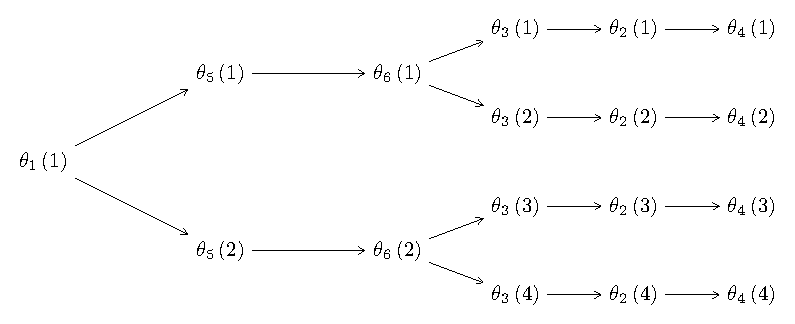
\includegraphics[width=0.435\textwidth, trim={0.01cm 0.01cm 0.01cm 0.01cm}, clip]{figures/Angle_Combination1.pdf}
	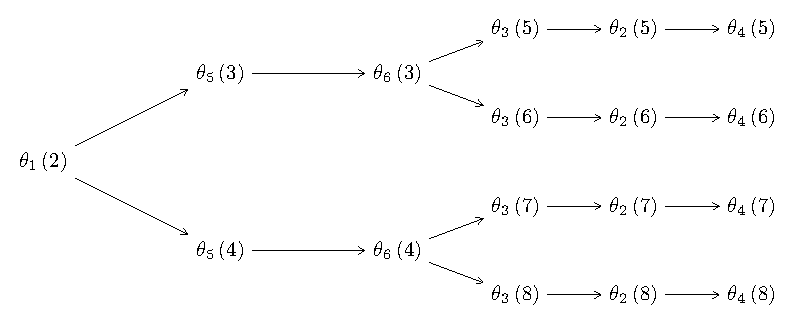
\includegraphics[width=0.435\textwidth, trim={0.01cm 0.01cm 0.01cm 0.01cm}, clip]{figures/Angle_Combination2.pdf}
	\caption{8 possible combinations of theta angles.}
	\label{Figure 1}
\end{figure}
The calculated desired joint angle combinations from inverse kinematics program must be modified before it can be used in further calculations as this could result in errors. This is accomplished by calculating three terms by adding factors 0, 2$\pi$, -2$\pi$ to each desired joint angle. The three terms are geometrically equivalent, but the robot would have to do one full rotation on this joint to get from one term to the next. Then the difference between the terms and the current robot position for each term is calculated. Afterwards, the factor resulting in the least difference is added to the desired angles. This procedure is repeated for all calculated desired joint angle values. \\
The best possible joint angles of the 8 possible combinations are chosen by calculating the overall absolute difference between each joint angle combination with the current pose of the robot. This overall absolute difference is calculated as the summation of the absolute values of the difference between each desired and the current joint angle. 
\begin{align*}
\mathrm{overall\,\,absolute\,\,difference\,\,for\,\,set} \,\, i = \sum\limits_{j=1}^6 \Delta\theta_j(i)\\
\Delta\theta_j(i) = \left| \theta_{j,current}-\theta_j(i) \right|
\end{align*}
Then the set of joint angles resulting in the least overall difference is chosen. This results in a more efficient transition of the robot between poses. 
\subsubsection{Implementation in ROS}
The overall task was implemented in ROS (Robot Operating System, a convenient middleware to control robots) since this brings many advantages: The overall program consist of multiple sub-programs called nodes, which can be programmed separately in different languages and communicate in a standardized way via ROS messages under certain so-called topics.\\
The implementation of kinematics was programmed in C++ and consists basically of two nodes, \textit{Direct Kinematics} and \textit{Inverse Kinematics}. There are principally two use cases: The Calibration (as needed for Task 2, marked in red) and the Head Movement Compensation (as needed for Task 4, marked in blue). Both use cases with their corresponding communication are illustrated in Figure \ref{fig:Nodes}. Nodes and objects which are needed in both use cases are marked in white.  The Direct Kinematics are used within the Calibration to get the current pose from the current joint angles. The Inverse Kinematics are used to calculate the desired joint angles for a desired position, which is given by either the Calibration or the Head Motion Compensation. Furthermore, we added one node called \textit{Move To Desired Angles}, which uses the result of the inverse kinematics and communicates this as a goal to the robot.\\
\begin{figure}[h]
	\centering
	\def\svgwidth{270pt}
	%\def\svgwidth{1\columnwidth} 
	\input{NodeOverview.pdf_tex}
	\caption{Node Overview. Nodes are shown in ellipses, other elements in rectangles. Messages are shown with solid lines, other relations with dashed lines.}
	\label{fig:Nodes}
\end{figure}
The nodes are built with this basic structure: In the main function an object of a class is created and a \textit{start}-function of that object is called. In this function, the ROS publishers and subscribers are created. The other parts of a node happen in so-called \textit{callback functions}. These functions are called whenever a new message is published to the relating topic.\\
For many nodes, the library \textit{Eigen} (Version 3) \cite{Eigen} was used. Eigen is an elegant and sophisticated solution to use matrices, vectors and quaternions in C++ because it contains corresponding arithmetic operations as well as conversions to other forms (e.g. quaternion to rotation matrix) and to ROS messages.
% ref to http://eigen.tuxfamily.org/

\subsection{Calibrations - FS}
\label{ssec:calib}
In order to compensate the motion of a patient both the pose of the patient and the coil have to be known at any time. For this reason, a RGBD camera is used that provides a point cloud from where a 3D scene can be reconstructed. Besides, a calibration between the camera reference frame and the robot base is needed to navigate the robot based on images from the camera. 
\subsubsection{Camera Calibration - JS}
Before the hand-eye calibration can be done, the camera itself needs to be calibrated. The goal of this calibration is to determine the parameters which are necessary to predict the pixels of the image of the objects in the field of view of the camera. Assuming the camera as a pinhole camera, the problem of calibration can be split up into two problems, the intrinsic and the extrinsic camera matrices.\\
The camera maps 3D points \textit{$M = (X,Y,Z)^T$} to 2D points \textit{$m =(u,v)^T$}. The vectors are augmented to \textit{$\tilde{M} = (X,Y,Z,1)^T$} and \textit{$\tilde{m} =(u,v,1)^T$}. The pinhole approach leads to the following matrices.
\begin{align*}
	\left.\begin{array}{r@{\mskip\thickmuskip}l}
	u = -\frac{fY}{Z}\\
	v = -\frac{fX}{Z}\\
	\end{array} \right\}
	\quad \implies \quad
  \left\{\begin{array}{r@{\mskip\thickmuskip}l}
	\begin{pmatrix}
		u\\
		v\\
		1
	\end{pmatrix}
	=
	\begin{pmatrix}
		\alpha&0&0\\
		0&\beta&0\\
		0&0&1
	\end{pmatrix}
	\begin{pmatrix}
		X\\
		Y\\
		Z
	\end{pmatrix}\\
	\end{array}\right.
\end{align*}
The intrinsic camera matrix \textit{A} describes the parameters intrinsic to the camera.
\begin{align*}
	A &= \begin{pmatrix}	\alpha& \gamma & u_0\\
											0& \beta& v_0\\
											0&0&1
	\end{pmatrix}
\end{align*}
This Matrix \textit{A} considers the offset of the image coordinates \textit{$(u_0,v_0)$}, the scaling factors \textit{$(\alpha,\beta)$} and a potential skew of the camera sensor \textit{$\gamma$}.\\
The extrinsic parameters \textit{$(R\ t) = (r_1\ r_2\ r_3\ t)$} are the rotational and translational parameters of the camera in regards to the world coordinate system.
With the intrinsic matrix \textit{A} and the extrinsic parameters \textit{(R, t)} the projection is given by:
\begin{align*}
	s\tilde{m} = A
	\begin{pmatrix}
		R&t
	\end{pmatrix}\tilde{M}
\end{align*}
with \textit{s} an scaling parameter.\\
Considering the planar calibration by Zhang \cite{camercalibrationzhang}, making the plane of the marker \textit{Z = 0} of the world coordinate frame system, this equation can be simplified to:
\begin{align*}
	s
	\begin{pmatrix}
		u\\v\\1
	\end{pmatrix}
	=A
	\begin{pmatrix}
		r_1&r_2&r_3&t
	\end{pmatrix}
	\begin{pmatrix}
		X\\Y\\0\\1
	\end{pmatrix}
		=A
	\begin{pmatrix}
		r_1&r_2&t
	\end{pmatrix}
	\begin{pmatrix}
		X\\Y\\1
	\end{pmatrix}
\end{align*}
Mutating the notation of \textit{M} to \textit{$M = (X,Y)^T$} thus \textit{$\tilde{M} = (X,Y,1)^T$} we can formulate the homography \textit{H}:
\begin{align*}
	s\tilde{m}=H\tilde{M}\ with\ 
	H =
	\begin{pmatrix}
	r_1&r_2&t
	\end{pmatrix}
\end{align*}

From an image with the two-dimensional marker, in this case a checkerboard, two constraints of the intrinsic parameters can be derived, as $r_1$ and $r_2$ of the homography \textit{H} are orthonormal.
\begin{align*}
h^T_2 A^{-T}A^{-1}h_2&=0\\
h^T_1 A^{-T} A^{-1} h_1&=h^T_2 A^{-T} A^{-1} h_2
\end{align*}
As the homography \textit{H} has 8 degrees of freedom 2 constraints on the intrinsic parameters can be determined by one homography. As there are five parameters in the intrinsic camera matrix \textit{A}, at least 3 images with different homographies are needed to determine all parameters. After calculating \textit{A} one is able to calculate all rotational and translational matrices with the used marker. Zhang also implemented a maximum likelihood estimation, minimizing the error between each point and its projection. \cite{camercalibrationzhang}
In this project the in the IAI Kinect2, a toolkit for the use of the Kinect v2 in ROS, included calibration tool was used to calibrate the intrinsic parameters of the RGB camera, the intrinsic parameters of the infrared camera, the extrinsic parameters of both cameras in relation to each other and finally the resulting depth data.\cite{iai_kinect2}
\subsubsection{Hand-Eye Calibration - FS}
The hand-eye calibration is used to get a relationship between the robot's reference frame and reference frame of the tracking device so that a navigation of the coil mounted at the robot's end effector based on images of calculated poses of the head is possible. For this reason we used an approach called \textit{QR24} which makes use of the relation \ref{fig:robtrac}:
\begin{align*}
\begin{array}{ll}
    (^RT_E)_i ^ET_M = ^RT_T (^TT_M)_i, & i=1,\dots,n
\end{array}
\end{align*}

\begin{figure}[!h]
	\centering
	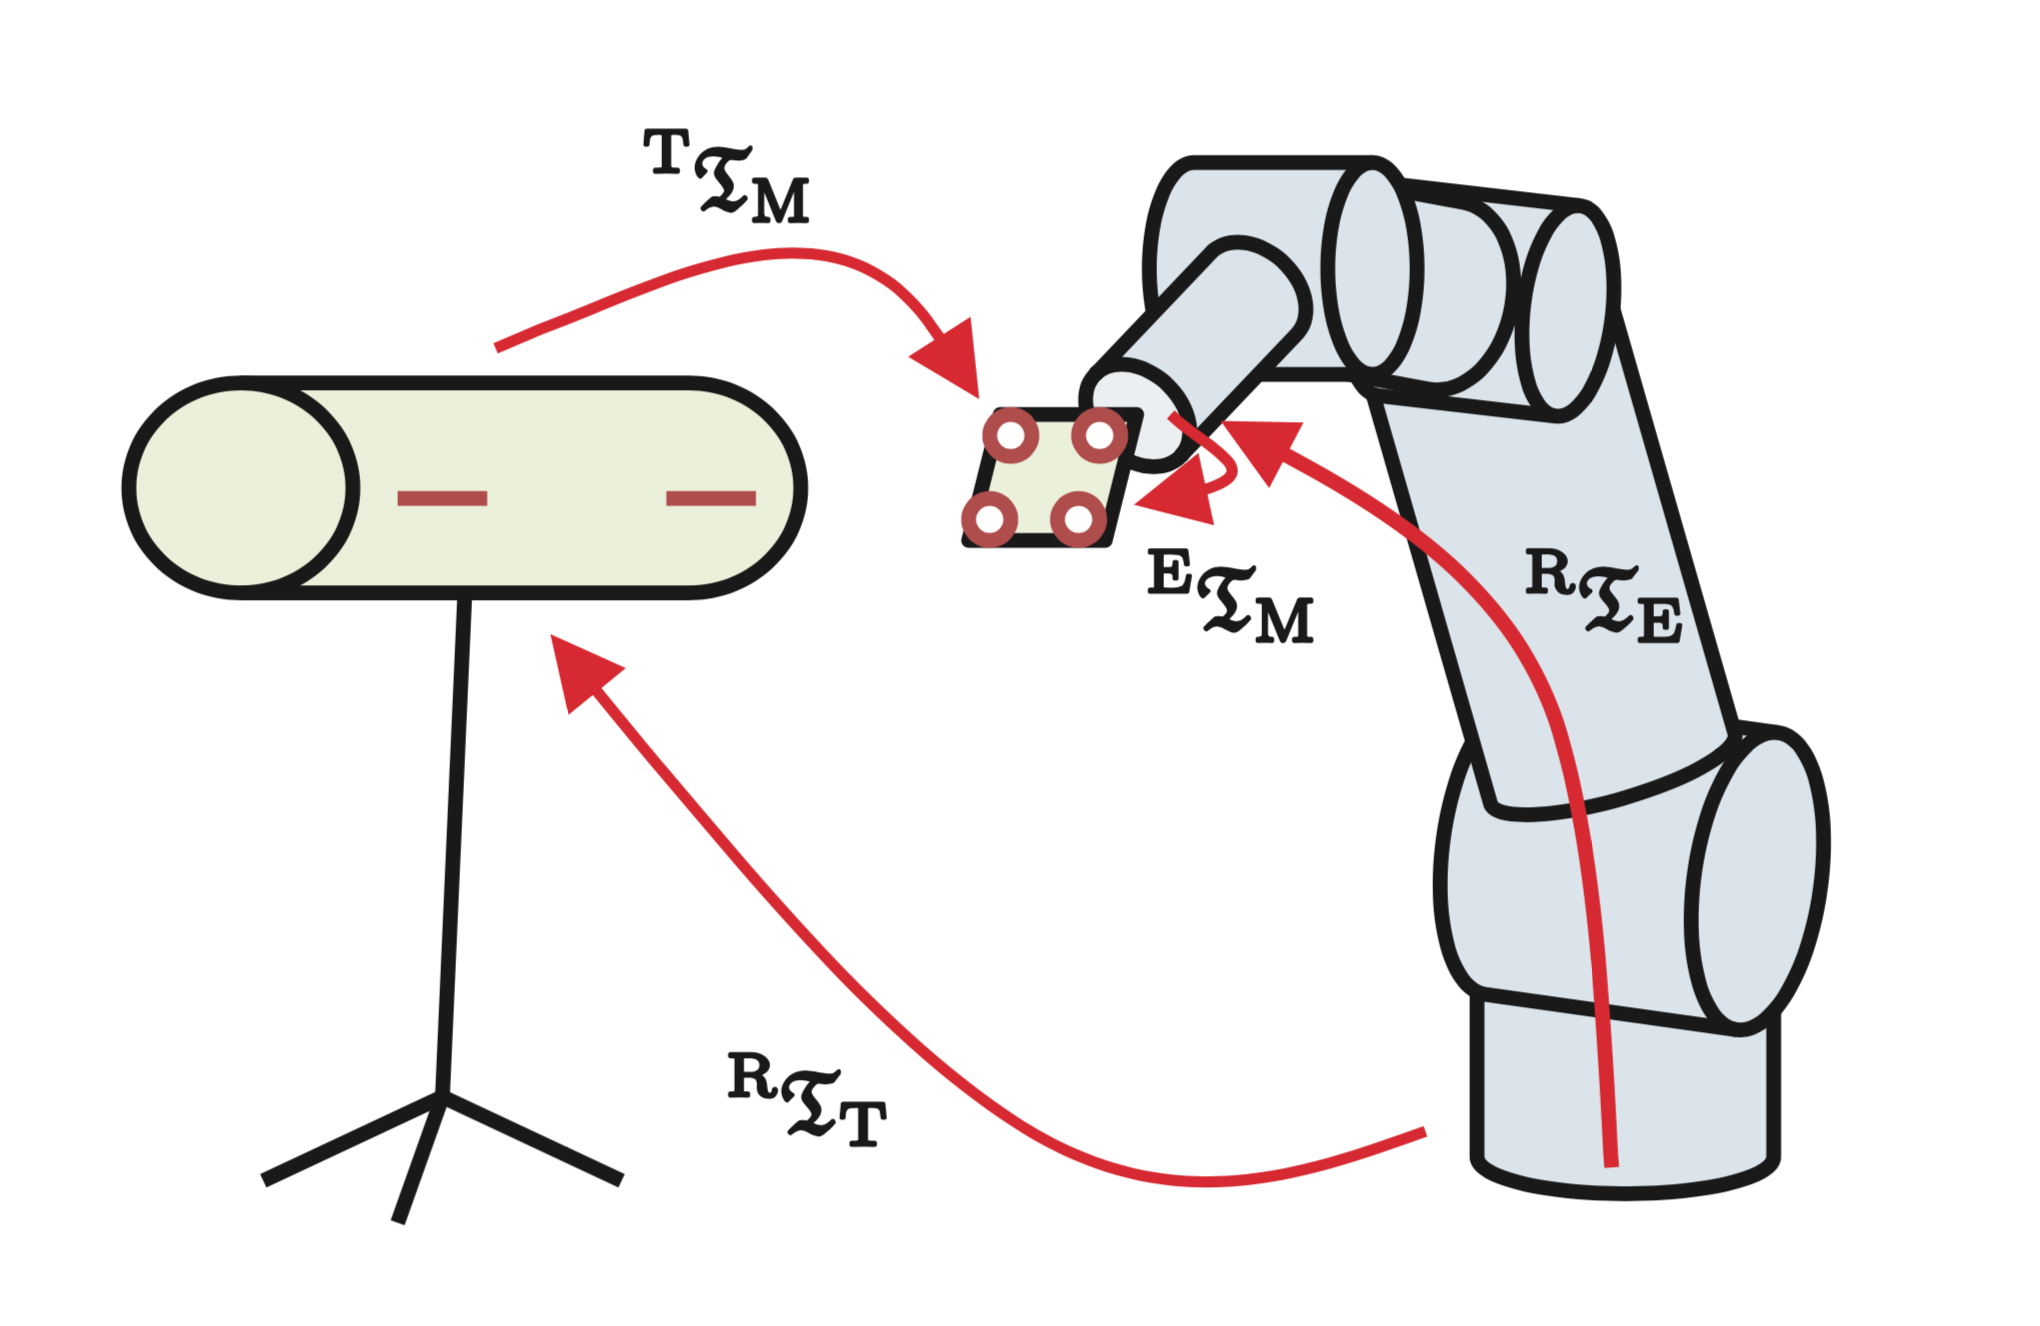
\includegraphics[width=0.35\textwidth]{figures/robot_tracker.png}
	\caption{Robot and optical tracking system \cite{ernst2012non}}
	\label{fig:robtrac}
\end{figure}
The robot's end effector is moved to random positions within a certain range for \(n\)-times \((^RT_E)_i\). At the end effector a checkerboard of known dimensions is mounted. For each of the the \(n\) poses an image is taken from which the pose of the checkerboard in relation to the camera reference frame is calculated \((^TT_M)_i\). With the collected data the desired transformation matrix \(^RT_T\) can be calculated using the least-squares approach \cite{ernst2012non}:
\begin{align*}
    \sum_{i=1}^n{\big|(^RT_E)_i ^ET_M - ^RT_T (^TT_M)_i\big|^2}
\end{align*}

\paragraph{Robot Poses - FS, GM, AU}
The robot starts in an initial pose \((^RT_E)_0\) manually set in which the checkerboard is both parallel and centered with respect to the tracking device. Out of this pose small changes in joint angles are made so that the end effector results in small changes in translation and rotation with respect to the robot base \((^RT_E)_i\):

\begin{alignat*}{2}
    d_i &= d_0 + \textit{rand}(\pm 10mm) &\qquad &\text{(translation)}\\
    \theta_i &= \theta_0 + \textit{rand}(\pm 10^\circ) &\qquad &\text{(angles)}\\
    R_i &= R_x(\theta _i)R_y(\theta _i)R_z(\theta _i) &\qquad &\text{(rotation)}
\end{alignat*}
\begin{align*}
\Rightarrow (^RT_E)_i &= \begin{pmatrix}R_i(0,0) & R_i(0,1) & R_i(0,2) & x_i\\
                                         R_i(1,0) & R_i(1,1) & R_i(1,2) & y_i\\
                                         R_i(2,0) & R_i(2,1) & R_i(2,2) & z_i
                                         \end{pmatrix}
\end{align*}

Here, \(d = \begin{bmatrix}x & y & z\end{bmatrix}^T\) and \(\theta = \begin{bmatrix}\theta_x & \theta_y & \theta_z\end{bmatrix}^T\) are vectors containing the translational part and the angles of \((^RT_E)\), respectively. \(R_{\cdot}(\theta)\) are the \(3\)x\(3\) elementary rotation matrices in \(x, y\) and \(z\) direction. The function \textit{rand(\(\cdot \))} creates different random values for each of the values in the vectors \(d\) and \(\theta\) within the given range. Small changes out of the initial position are important to maintain consistency with the tracking device, i.e. it is possible to calculate the pose of the checkerboard out of the images \((^TT_M)_i\) (see \ref{par:Marker Positions - JS}). If it is not possible to get the pose of the checkerboard \((^TT_M)_i\) for a certain configuration \((^RT_E)_k\) of the robot, a new pose will be generated, the non-consistent pose will be overwritten and the algorithm to get the pose of the checkerboard will be told to try again. After \(n\)-iterations a matrix of \(4n x 4\) consistent transformation matrices has been generated. 


\paragraph{Marker Positions - JS}
\label{par:Marker Positions - JS}
The Marker Positions are recorded via a python script. A ROS node is implemented, which waits for the in figure \ref{fig:Nodes} shown order to take images. As soon as the robot reaches its final pose the script tries to detect the used marker and takes numerous pictures of the current pose of the robot. The as the marker used checkerboard is detected via corner detection of the OpenCV library \cite{opencv}. For the image the already rectified images with the in the camera calibration used distortion coefficients are used for the ease of post processing of the images. The to the topic /kinect2/sd/image\_ir\_rect and /kinect2/sd/image\_depth\_rect posted images are used, as the resolution of 512x424 pixel is the maximum output of the Kinects depth stream.\cite{kinectresol}\\ The time synchronized pictures of the image stream are used and saved.
After the desired number of pictures were taken, or for a prolonged time no checkerboard was detected, the script reports into a topic that it is done and the robot can move to a new pose and afterward the script tries to take the next series of images.\\
After the desired number of poses have been run through and the images are saved, the transformation matrices for the tracker to checkerboard matrices \((^TT_M)_i\) are to be calculated. Therefore again the pixels \textit{$u_i,\ v_i$} with the checkerboard corners are detected. To remove the signal noise in the depth image, averaging about the in a single pose taken depth images is done, the depth values \textit{$d_i$} are, through the calibration, related to the pixels \textit{$u_i,\ v_i$} in the infrared image. The 3D pose of the checkerboard can now be estimated with the use of the intrinsic camera parameters \textit{A}
\begin{align*}
X_i &= \frac{u_i-u_0}{\alpha}*d_i\\
Y_i &= \frac{v_i-v_0}{\beta}*d_i\\
Z_i &= d_i
\end{align*}
Finally the tracker to checkerboard matrices \((^TT_M)_i\) are calculated via least-square estimation by the Umeyama-Method.\cite{umeyama}

\paragraph{QR24-Algorithm - FS}
After the corresponding transformation matrices of \(n\) configurations of the robot \((^RT_E)=M\) and consistently to these poses \(n\) poses from the tracking system to the checkerboard \((^TT_M)=N\) have been generated, it is possible to find the optimal entries of static transformation matrices from robot base to the tracking device \(^RT_T=Y\) and from the end effector to the marker position \(^ET_M=X\) in terms of minimizing the quadratic error:
\begin{equation*}
\label{eq:qr24}
    \sum_{i=1}^N{|M_i X - Y N_i|^2} 
\end{equation*}
These two matrices have both \(12\) non-trivial elements that can be combined into a vector \(w = \begin{bmatrix}x_{1,1},x_{2,1},\dots, y_{1,1},y_{2,1},\dots,y_{3,4}\end{bmatrix}^T \in \mathbb{R}^{24} \). Thus, at least 24 poses are needed to estimate the elements of \(w\). The equation \eqref{eq:qr24} can be combined to a system of linear equations \(Aw = b\) to find the optimal solution of \(w\)\cite{ernst2012non}.\\
For minimizing the error and thus getting a sufficient result more poses than \(24\) are eventually needed. However, there is a chance of overfitting as well, i.e. the estimated matrix has good results with the training data but has poor generalization abilities with new poses. For this reason, the data is split into training and test data, respectively. 80\% of the data was used for training and the remaining 20\% was used to test whether the error is small enough. 
\paragraph{Evaluation QR24 - FS}
The implementation was initially intended to be in Python which gets the matrices \(M_i\) and \(N_i\) to build \(A\) and \(b\) and calculates \(w\) from where \(X\) and \(Y=\,^RT_T\) can be build. However, when it came to testing at the end of the project the Python solution was inconsistent with another estimation known to be good. From this perspective it was not clear whether the mistake was in the \textit{QR24} algorithm, in the kinematics or in marker pose estimation.\\
To test the \textit{QR24} algorithm a model of known dimensions and outcomes has been generated via Matlab. The model was constructed to be most similar to the real scenario, i.e. small changes in the robot parameters resulting in different robot configurations \((^RT_E)_i\) from where the corresponding transformation matrix from the tracking device to the marker position \((^TT_M)_i = (^RT_T)^{-1}\, (^RT_E)_i\,^ET_M\) can be calculated. This is working since \(^RT_T\) and \(^ET_M\) are initially known in this model. Nevertheless, out of the generated data \((^RT_E)_i\) and \((^TT_M)_i,\,i=1,\dots,1000\) the matrices \(^RT_T\) and \(^ET_M\) are estimated using the \textit{QR24} approach and compared to the real target values. \\
Here, similar implementations of the algorithm has been realized in both Python and Matlab. After discovering and correcting a mistake in  building the matrix \(A\) in the initial Python code the outcomes of the orthonormalized matrices \(^RT_T\) where the following:

\begin{align*}
^RT_{T_{\text{target}}} &= \begin{bsmallmatrix}1 &&&&&& 0 &&&&&& 0 &&&&&& 8 \\
                   0 &&&&&& 1 &&&&&& 0 &&&&&& 0 \\
                   0 &&&&&& 0 &&&&&& 0 &&&&&& 0 \\
                   0 &&&&&& 0 &&&&&& 1 &&&&&& 1 \end{bsmallmatrix} \\
^RT_{T_{\text{phyton}}} &= 
    \begin{bsmallmatrix}1 & 2.45\cdot 10^{-8} & -2.54\cdot 10^{-7}& 7.99 \\
                   -2.45\cdot 10^{-8} & 1 & 3.27\cdot 10^{-8} & -1.10\cdot 10^{-6} \\
                   -2.54\cdot 10^{-7} & -3.27\cdot 10^{-8} & 1 & 8.36\cdot 10^{-6} \\
                   0 & 0 & 1 & 1 \end{bsmallmatrix}\\
^RT_{T_{\text{matlab}}} &= 
    \begin{bsmallmatrix}1 & -1.02\cdot 10^{-15} & 5.07\cdot 10^{-16}& 8.00 \\
                  1.02\cdot 10^{-15} & 1 & -3.05\cdot 10^{-16} & -2.58\cdot 10^{-15} \\
                  -5.07\cdot 10^{-16} & 3.33\cdot 10^{-16} & 1 & -4.51\cdot 10^{-15} \\
                   0 & 0 & 1 & 1\end{bsmallmatrix}             
\end{align*}

The residual sum of squares (RRS) is the square sum of the differences between the target values and estimated values of each entry in the matrices which is used to measure the discrepancy between the data and the estimated model:
\begin{align*}
RSS &= \sum_{i=1}^4\sum_{j=1}^4 (^RT_{T_{\text{tar}}}(i,j) - ^RT_{T_{\text{est}}}(i,j))^2
\end{align*}
For the modeled data the RSS are:
\begin{center}
\begin{tabular}{l|r}
Python & \(1.32\cdot 10^{-10}\) \\
Matlab & \(3.30\cdot 10^{-29}\)
\end{tabular}
\end{center}
It can be seen that the algorithm works really well in Matlab but seems to have some issues by using python's environment \textit{numpy} for solving the linear equation.\\
For the data we collected during the project the matrices are the following:

\begin{align*}
^RT_{T_{\text{target}}} &= \begin{bsmallmatrix}0.6940 && -0.1306 && 0.7079 &&	-1.0052 \\
-0.7192 &&	-0.0834 && 	0.6897 && 	-0.5073 \\
-0.0310 && 	-0.9879 &&  -0.1518 && 	0.4933 \\
0 && 0 && 	0	&& 1\end{bsmallmatrix} \\
^RT_{T_{\text{phyton}}} &= 
    \begin{bsmallmatrix}
    0.0268 &&	0.0133 &&	0.0254 &&	-0.3645 \\
    -0.0216 &&	0.0041 &&	0.0182 &&    -0.0698 \\
    0.0150 &&   -0.0305 &&    0.0016 &&	0.50216 \\
    0 &&	0 && 0 && 1
     \end{bsmallmatrix}\\
^RT_{T_{\text{matlab}}} &= 
    \begin{bsmallmatrix}
    0.5542 &&	0.7797 &&	0.2912 &&	-0.0020 \\
    0.0991 &&   -0.4092 &&	0.9070 &&	-0.0002 \\
    0.8264 &&   -0.4738 &&	-0.3041 &&	0.0031 \\
    0 &&	0 &&	0 &&	1
     \end{bsmallmatrix}             
\end{align*}
The RSS results are:
\begin{center}
\begin{tabular}{l|r}
Python & \(3.4212\) \\
Matlab & \(4.3716\)
\end{tabular}
\end{center}
The error with the collected data is still huge. In conclusion, there must be another error either in the calibrations or in the pose estimation of the target.  

\subsection{Head Tracking - CG}
For motion compensation the head pose needs to be estimated. Therefore, the head first needs to be localized. This can be done by identifying the area of depth which contains a head. The authors \cite{headtracking} propose an adaptive detection filter where the size depends on the expected size of the head at various depths. They assume that the focal length is known and that only one head is present in the scene. Moreover, the subject is supposed to be at depth between $d_m$ and $d_M$ so that a binary mask $\epsilon (i,j)=d_m<d_0(i,j)<d_M$ can be used. The expected width $w(i,j)$ and height $h(i,j$ of the head are centered at $(i,j)$. A score $s(i,j)$ is obtained by resizing the kernel and convolving it with the binary mask $\epsilon(i,j)$. The maximum scored pixel gives the center of the identified head and therefore the full head location by using width and height at that pixel. The authors choose a larger region of interst so that the head is fully contained in the process \cite{headtracking}.

For the head pose estimation, the authors divide the process into a reference model, a cost function, optimization and morphable model fitting. For the reference model the provided head model can be used. The facial surface is chosen as set of 3d vertices. Mismatches are considered as weight factor for the surface. The cost function models the head pose in 6d consisting of position and orientation and quantifies the difference between the observed and hypothetical data by factoring out the effects of outliers. For optimization particle swarm optimization and iterative closest point are used. The trade-off between accuracy and computation time needs to be considered. In the last step, the shape and weights of the morphalbe model are updated and point correspondences are identified to compute a new set of coefficients of the morphable model \cite{headtracking}.

In our project, we initially used an open source code based on the approach of Fanelli et al \cite{head_pose_estimation}.
This approach estimates the head pose from given depth data and is based on discriminative random regression forests. That is training combinations of random trees by splitting the nodes so that the entropy of the label distribution and the variance of the head position and orientation are reduced \cite{head_pose_estimation}.
Unfortunately, this algorithm did not work for our problem since the used point clouds have a different structure than the used data of our head model.


\subsection{Motion Compensation}
The last task consisted of three smaller subtasks which will be discussed individually.
\subsubsection{Initial Path Planning}
This task asked for path planning for the initial coil pose to avoid hitting the head. Since this was an optional task, our group decided to focus on the other tasks and rather get these working. Therefore, we did not include path planning.
\subsubsection{Trajectory Planning - GM}
Trajectory planning is about how fast a movement should happen. It describes the position, velocity and acceleration as a function of time. For this, there are many different approaches, such as cubic splines, LSPB or Bang-Bang Control (which requires the least amount of time).
Since there is a post-processing of trajectories happening in the robot software, we decided not to include Trajectory Planning and set the corresponding variable \textit{traj\_time} to $0.01\,s$.
Nevertheless, we considered using Trajectory Planning at first. Our general idea was to identify the slowest movement of the six joints and take this as the time in which all movements should happen.\\
The approach of this idea can be found in the move-node under the keyword \textit{Approach for trajectory planning (not used)}[which is commented out since we did not use it], although the last command to assign \textit{traj\_time} to the value of \textit{T\_tmp} is missing.
\subsubsection{Motion Compensation - FS, AU}
The motion compensation system brings all individual parts together. First, the head pose is tracked by the Kinect camera to get \(^KT_H\). With this information a new goal pose of the coil can be calculated since the matrices from end effector to head \(^ET_H\) and from the robot base to the Kinect camera \(^BT_K\) are known \ref{ssec:calib}. 

\begin{alignat}{2}
    ^BT_E &=\,^BT_K \, ^KT_H \, ^HT_E &\qquad &\text{(new goal)}
\end{alignat}

This matrix is sent to the inverse kinematics (see fig. \ref{fig:Nodes}). This is repeated during the whole TMS process. 

\section{Conclusion \& Evaluation - GM}
The overall task was to create a vision-guided robot system to achieve head movement compensation for transcranial magnetic stimulation. This was done in four tasks, namely the robot kinematics, the calibration of the camera, the head movement estimation and the combination of the latter three tasks to compensate head movement. To test the setup a styrofoam head was mounted on a separate robot and made unknown movements the motion compensation system needed to compensate. As mentioned before neither the hand-eye calibration nor the head tracking were functioning at this moment of time. Thus, these parts were replaced by given algorithms to test the remaining parts. One was able to see with the bare eye that there was a delay in the movement (guessing it is around $0.5\,s$). Due to the sophisticated structure of the evaluation data, we were not able to evaluate the results quantitatively. We tried to by using the rosbag package as well as the provided .py file, but it was not feasible for us to understand it well enough in time.




% conference papers do not normally have an appendix


% use section* for acknowledgment
\section*{Acknowledgment}

The authors would like to thank the Institude of Medical Technology for the great support during the group project. Especially, we would like to thank Omer Rajput and Mareike Wendebourg for the helpful consultations even out of our lab times.





% trigger a \newpage just before the given reference
% number - used to balance the columns on the last page
% adjust value as needed - may need to be readjusted if
% the document is modified later
%\IEEEtriggeratref{8}
% The "triggered" command can be changed if desired:
%\IEEEtriggercmd{\enlargethispage{-5in}}

% references section

% can use a bibliography generated by BibTeX as a .bbl file
% BibTeX documentation can be easily obtained at:
% http://www.ctan.org/tex-archive/biblio/bibtex/contrib/doc/
% The IEEEtran BibTeX style support page is at:
% http://www.michaelshell.org/tex/ieeetran/bibtex/
\bibliographystyle{IEEEtran}
% argument is your BibTeX string definitions and bibliography database(s)
%\bibliography{IEEEabrv,../bib/paper}
\bibliography{IEEEexample}

%
% <OR> manually copy in the resultant .bbl file
% set second argument of \begin to the number of references
% (used to reserve space for the reference number labels box)
%\begin{thebibliography}{1}
%
%\bibitem{IEEEhowto:kopka}
%H.~Kopka and P.~W. Daly, \emph{A Guide to \LaTeX}, 3rd~ed.\hskip 1em plus
  %0.5em minus 0.4em\relax Harlow, England: Addison-Wesley, 1999.
%
%\end{thebibliography}




% that's all folks
\end{document}


